\documentclass[a4paper, 10pt]{article}


\usepackage[slovene]{babel}
\usepackage[utf8]{inputenc}
\usepackage[T1]{fontenc}
\usepackage{amsmath}
\usepackage{graphicx}



\begin{document}
\newtheorem{example}{Zgled}
\newtheorem{theorem}{Izrek}
\newtheorem{proof}{Dokaz}
\newtheorem{definition}{Definicija}
\newtheorem{lemma}{Lema}



\title{Odpornost snarkov}
\author{Vanja Kalaković in Eva Strašek}
\maketitle

\pagebreak

\section{Uvod}

Najprej bomo opredelili, kaj snarki sploh so.

\begin{definition}
    Če so vsa vozlišča grafa G enake stopnje k, pravimo, da je graf
k-regularen; 3-regularnim grafom pravimo tudi kubični graf.
\end{definition}

\begin{definition}
    Predpostavimo, da imamo graf $G = (V,E)$. Odpornost povezav $er(G)$ je velikost najmanjšega
    cikličnega prereza grafa $G$. Graf je ciklično $k$-povezan, če je $er(G) \ge k$, kar 
    pomeni, da moramo grafu G, odstraniti najmanj $k$ povezav, da nam ta razpade na dve 
    komponenti, ki vsebujeta ta cikel.
\end{definition}

\begin{definition}
    Predpostavimo, da imamo graf $G = (V,E)$. Odpornost vozlišč $vr(G)$ je najmanjše število $k$
    vozlišč $E$, ki jih je treba odstraniti, da postane graf $G$ $k$-robno obarljiv.
\end{definition}

\begin{definition}
    Snark je ciklično 4-povezan kubičen graf z notranjim obsegom vsaj 5 in 
    kromatičnim indeksom 4. Snark reda $n$ in velikosti $m$ označimo z $S(n,m)$.
\end{definition}

\begin{figure}[h]
    \centering
    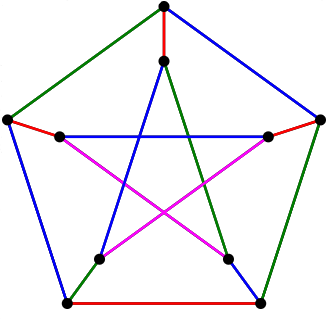
\includegraphics[scale=0.5]{Petersenov_graf1}
    \caption{Petersenov graf je najmanjši snark. Vsi snarki vsebujejo subdivizijo Petersenovega grafa}
\end{figure}

\section{Načrt dela}

\subsection*{Navodilo:}
Prenesite nekaj majhnih snarkov iz House of Graphs in
poskusite odgovoriti na naslednje vprašanja.
\begin{itemize}
    \item Primerjajte $vr(G)$ in $er(G)$.
    \item Poišči najmanjši snark z $vr(G) \ge 3$.
\end{itemize}

\subsection*{Načrt dela:}
Najprej bova napisali program, ki bo izračunal odpornost vozlišč $vr(G)$ in program, ki bo 
izračunal odpornost povezav $er(G)$ za snarke, ki jih boma prenesli iz House of Graphs.
Nato bova primerjali odpornost vozlišč in odpornost povezav danih snarkov. Pri odstranjevanju
vozlišč in povezav moramo paziti da program odstranjuje naključne povezave ali vozlišča, zato 
je boljše, da ga večkrat ponovimo in izberemo najmanjše število.






\end{document}